%%%%%%%%%%%%%%%%%%%%%%%%%%%%%%%%%%%%%%%%%%%%%%%%%%%%%%%%%%%%%%%%%%%%%%%%%%%%%%%%
%
% A Template for Trace Documents
% 
% This is a template for producing TRACE documents according to:
%
% Grimm V, Augusiak J, Focks A, Frank B, Gabsi F, Johnston ASA,  
% Liu C, Martin BT, Meli M, Radchuk V,  Thorbek P, Railsback SF. 2014. 
% Towards better modelling and decision support: documenting model development, 
%  testing, and analysis using TRACE. Ecological Modelling  
%
% and
%
% Augusiak J, Van den Brink PJ, Grimm V. 2014. Merging validation and evaluation of 
% ecological models to `evaludation': a review of terminology and a practical
%  approach. Ecological Modelling. 

% Before you compile a TRACE document, please read the above two publications, plus:

% Schmolke A, Thorbek P, DeAngelis DL, Grimm V. 2010. Ecological modelling supporting 
% environmental decision making: a strategy for the future. 
% Trends in Ecology and Evolution 25: 479-486.

% In the template, text in < > provides instructions and explanations and should be 
% replaced by your own text. By filling in your own text, tables, figures, and 
% hyperlinks, and by deleting instructions and explanations, you can create your 
% own TRACE document. 

% Please keep the short explanation that is given at the begin of each TRACE element; 
% it will remind you and readers what this element is about.

% We recommend keeping the simplistic formatting of this file so TRACE documents 
% produced by different authors not only use the same structure and terminology, 
% but also look similar, making it easier for model users to perceive TRACE as a 
% standard format.

% TRACE documents are designed to be supplementary material provided in electronic 
% and/or printed form to add credibility to your model and its results. Please refer 
% in your main article or report, where you present the model and its application, 
% to the TRACE document in the following way:

% ``In the Supplementary Material, we provide a TRACE document ("TRAnsparent and 
% Comprehensive model Evaludation''; Schmolke et al. 2010; Grimm et al. 2014; 
% Augusiak et al. 2014) containing evidence that our model was thoughtfully designed, 
% correctly implemented, thoroughly tested, well understood, and appropriately used 
% for its intended purpose. A summary of the TRACE document is given in Table <..>."

% It is important that you refer to those publications so that model users can check 
% whether you followed the standard defined in Grimm et al. (2014), that they 
% understand the rationale of TRACE (Schmolke et al. 2010) and of model evaludation 
% (Augusiak et al. 2014); it also allows the developers of TRACE to scan the 
% literature for consistent use of TRACE, which is important for future refinements.
% See also: http://cream-itn.eu/trace 
% When producing your TRACE document, delete this first page.

%% End of MS Word Template's first page
%%%%%%%%%%%%%%%%%%%%%%%%%%%%%%%%%%%%%%%%%%%%%%%%%%%%%%%%%%%%%%%%%%%%%%%%%%%%%%%%%%%%%%
%% 
%% This document template was created by Richard A. Erickson.
%% Please feel free to contact him with any suggestions, tips, or improvements.
%% He may be reached at raerickson@gmail.com
%% Note that this template is provided without warranty and as is. However, he would
%% gladly take suggestions for improvement and would be happy to collaborate on 
%% creating a .sty file or improving documentation for this template.  
%%
%% LaTeX notes, suggestions, and tips:
%% 0) This document assumes the user is familiar with LaTeX basics.
%% 1) The PDF produced by this does not exactly follow the Word template because 
%%    because some of the suggestions in the Word template are included as 
%%    comments in the LaTeX template. 
%% 2) Conversely to point 1, some directions were copied over directly from the Word 
%%    file and may not make sense with LaTeX.
%% 3) The optional sectional table of contents requires is only included for section 1.
%%    If you desire TOC for other sections, simply copy and paste this example code. 
%% 4) I would suggest using the url package to include url links.
%% 5) Recall the \label{} and \ref{} functions to reference objects within the code.
%% 6) You'll need to include figures with the figures environment. I do not provide examples
%%    Within this document.



\documentclass{article}[12pt]
\usepackage[letterpaper, margin=1in]{geometry} % used to set margins and specify page size
\usepackage{fancyhdr} % used to create headers 
\usepackage{titlesec} % Used to change section headers
\usepackage{titletoc} % needed for the sectional table of contents
\usepackage{url}
\usepackage{natbib} % Used for citations
\usepackage[nottoc]{tocbibind}
\usepackage{setspace}
\usepackage{graphicx}
\usepackage{subcaption}
\usepackage{tocloft}
\usepackage{parskip}
\usepackage{amsmath}
\usepackage{amssymb}
\usepackage{topcapt, booktabs} % used for tables
\renewcommand{\cftsecleader}{\cftdotfill{\cftdotsep}}


\onehalfspacing

\titleformat{\section}
{{\titlerule[0.8pt]}\normalfont\Large\bfseries}{\thesection}{1em}{}[{\titlerule[0.8pt]}]

\setlength{\parindent}{0pt}

\pagestyle{fancy}
\fancyhf{}

\chead{TRACE document: Erickson et al. YY-male grass carp IPM}
\cfoot{\thepage}

\begin{document}

\begin{center}
\textbf{{\huge TRACE document}}
\end{center}

 This is a TRACE documentation (``TRAnsparent and Comprehensive model Evaludation''), 
which provides supporting evidence that our model presented in:
\begin{center}
\textbf{Erickson RA, Eager EA, Bray MK, Hansen MJ, and Kocovsky PM. An integral projection model with YY-males and application to evaluating grass carp control. Ecological Modelling.}
\end{center}
was thoughtfully designed, correctly implemented, thoroughly tested, well understood, and appropriately used for its intended purpose. 

 The rationale of this document follows: 
\begin{verse}
Schmolke A, Thorbek P, DeAngelis DL, Grimm V. 2010. Ecological modelling supporting environmental decision making: a strategy for the future. \textit{Trends in Ecology and Evolution} 25:479-486.
\end{verse}
and uses the updated standard terminology and document structure in:
\begin{verse}
Grimm V, Augusiak J, Focks A, Frank B, Gabsi F, Johnston, Liu C, Martin BT, Meli M, Radchuk V, Thorbek P, Railsback SF. 2014. Towards better modelling and decision support: documenting model development, testing, and analysis using TRACE. \textit{Ecological Modelling} 280:129-139
\end{verse}
and
\begin{verse}
Augusiak J, Van den Brink PJ, Grimm V. 2014. Merging validation and evaluation of ecological models to `evaludation': a review of terminology and a practical approach. \textit{Ecological Modelling}. 280:117-128
\end{verse}


\pagebreak

% \dominitoc % Initialization
\tableofcontents

\pagebreak
\section{Problem Formulation}
\textbf{This TRACE element provides supporting information on:} The decision-making context in which the model will be used; the types of model clients or stakeholders addressed; a precise specification of the question(s) that should be answered with the model, including a specification of necessary model outputs; and a statement of the domain of applicability of the model, including the extent of acceptable extrapolations. 

\textbf{Summary:}
\begin{verse}
\textbf{
Grass carp (\textit{Ctenopharyngodon idella}) are native to eastern Asia.
The fish have been transported outside of their native range for weed control and have escaped into native habitats. 
As an invasive species, grass carp disrupt native ecosystems and vegetation. 
Controlling the species is important for conservation biology and fisheries management. 
Population models are one tool for guiding carp control efforts and better understanding carp life history. 
Possible management activities include containment through barriers, harvest, releasing YY-males, and developing carpicides.  
All of these approaches would benefit from population models to guide management. 
The objective of our model is assist in the control of grass carp. 
The objective of the corresponding paper is to present and analyze our model.
We also apply the model to compare different management scenarios with YY-males.
}
\end{verse}

Grass carp are native to castern Asian and range from the Amur River of eastern Russia to the West River of southern China \citep{shireman1983synopsis}.
The range also gives it another common name, white Amur.
The species feeds on aquatic vegetation and has been introduced around the world, including Malaysia, Taiwan, Japan, easter Europe, Holland, German, and the United States of America \citep{cross1969aquatic}.
Although effective at weed control, the species has also escaped into the wild and disrupts native ecosystems \citep{chapman2013first}.
The species decimates native macrophyte communities, which in turn alter ecosystem function, habitat structure, community process, and food web dynamics \citep{dibble2009ecological}.
Within North America, grass carp were first proposed to be released in 1957 \citep{swingle:1957} and first released six years later \citep{bain1993assessing}.
Grass carp quick spread from release sites and have dispersed to other  systems including the Mississippi River \citep{bain1993assessing} and Great Lakes \citep{chapman2013first} (Figure \ref{fig:carpMap}).


\begin{figure}[htbp]
   \centering  
   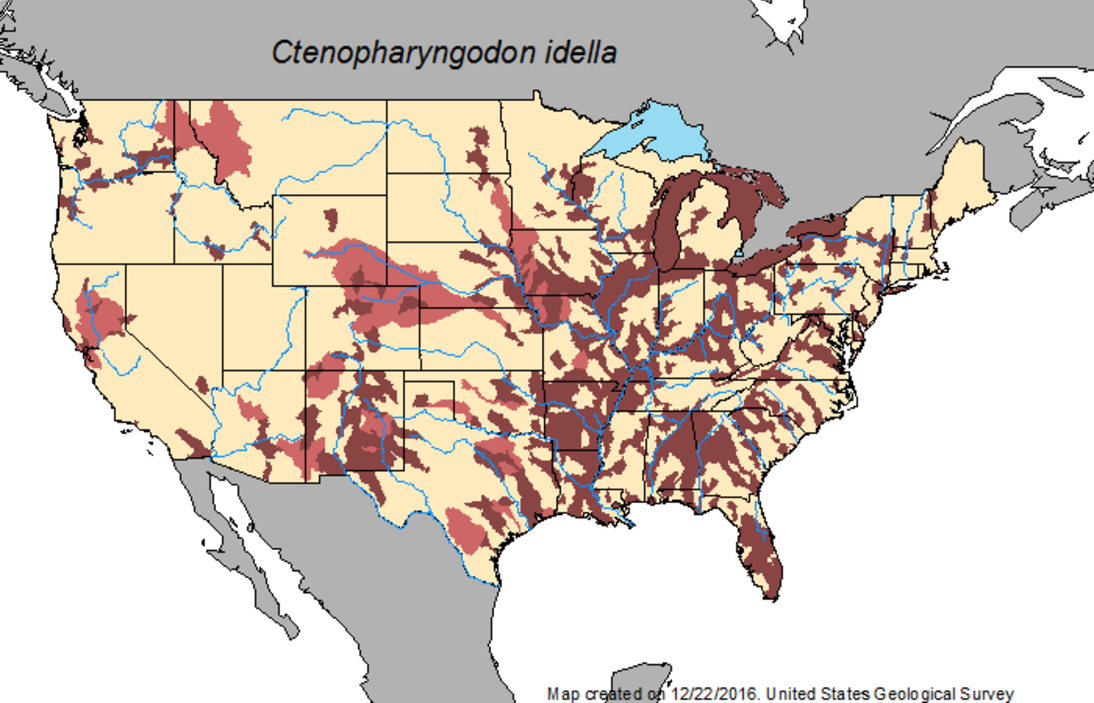
\includegraphics[width=0.75\textwidth]{carpMap.pdf} % requires the graphicx package
   \caption{Species distribution map of grass carp (\textit{Ctenopharyngodon idella}) in the continental United States. Map is was generated by the USGS on 22 December 2016 and accessed 23 January 2017 (\protect\url{https://nas.er.usgs.gov/queries/factsheet.aspx?SpeciesID=514}). The figure was created by Nico, L.G., P.L. Fuller, P.J. Schofield, M.E. Neilson, A.J. Benson, and J. Li while working for the US Government and is in the public domain.}
   \label{fig:carpMap}
\end{figure}

Grass carp management has changed in the United States and North America through time. 
Initial management of grass carp actually focused on increasing individual survival because the species was (and still is to some) a desirable aquatic weed control species \citep[e.g.,][]{cross1969aquatic, mitzner1978evaluation, kilambi1979effects, rottmann1991comparison}.
Shortly after the first grass carp were introduced to North America, managers noted adverse effects of grass carp and the introduction of sterile individuals (e.g., triploids) were used to limit the impact of introduced carp \citep{chilton1992biology}.  
Management of grass carp  in many areas of North America has now changed to focusing on limiting invasions, monitoring invasion, and controlling the species \citep{chapman2013first, wittmann2014grass}. 
Several different species of carp have been introduced to North America and control techniques developed for these and other fishes may also be applicable to grass carp as well.
Possible tools include acoustical conditioning \citep{sloan2013acoustical},
new carpicides \citep{putnam2017using},
commercial harvest \citep{colvin2012strategies},
and the release of YY-males that only produce male offspring \citep{schill2016production}.
Prior to the expensive development and implementations of these and other possible management options, managers and researchers may wish to evaluate the effectiveness of the approaches. 
Mathematical models are one method for running ecological simulations \citep{bolker2008ecological}.
Additionally, mathematical theory can be applied to ``optimize'' management \citep{lenhart2007optimal} or at a minimum, allow different management strategies to be compared \citep{caswell_matrix_2001, morris2002quantitative}.

Mathematically, several population models have been developed for invasive carp \citep[e.g., silver carp, bighead carp, common carp;][]{lorenzen1995population, williamson2005growth, tsehaye2013prospects,cuddington2014could} including grass carp \citep{kirk2000population}.
The life history of carps (family Cyprinidae) is likely conserved enough that these models could be re-parameterized for grass carp and \citet{lorenzen1995population} presents a generic fisheries model that includes carps.
However, these models are not applicable to our management questions. 
First, the models tend to be designed for specific locations and questions that differ from ours.
Second, none of these models differentiate carp by sex nor do they include YY-males.
Last, the grass carp model \citet{kirk2000population} does not include sufficient details to reproduce the model, highlighting the need for documentation such as TRACE and ODD \citep{schmolke2010ecological, augusiak2014merging}.
These modeling gaps point to the need for a new carp model that can be readily adapted to new management scenarios. 
Our model was designed to explore different population-level management options of grass carp by resource managers.
Possible organizations that might use our model include international organizations (e.g., the Great Lakes Fisheries Commission), national management agencies (e.g., the US Army Corps of Engineers, the US Fish and Wildlife Service, Environment Canada), state/provincial agencies, and other groups (e.g., NGOs, local governments). 
The model could also be used to help guide conservation of the species in its native range, where the species has declined due to overfishing \citep{shireman1983synopsis}

As an additional modeling consideration, previous models have tended to be difference equations or differential equations that discretize carp size (e.g., matrix models) or ignore size/age structure. 
However, carp, like most fish, grow continuously and change in size through time. 
Hence an integral projection model would more accurately reflect the life history of the species \citep{ellner2006integral, ramula2009integral, merow2014advancing}. 


Our model produces two state-variables for a population: the population number (e.g,. 1,000 carp at year 10) and the population size distribution (e.g., the length of the fish at year 10 was a binomial distribution with modes at\ldots).
We specifically designed the model to answer the following question:
\begin{enumerate}
\item How many YY-males must be released to cause quasi-extinction for a population? and
\item How long will the stocked males persist in the environment?
\end{enumerate} 
Answering these questions will help managers evaluate the potential for using YY-males to control grass carp.  

% \textbf{Summary contents \(<\)Optional table of contents\(>\)}
% \startcontents[sections]
% \printcontents[sections]{ }{2}{}

% \stopcontents[sections]

\section{Model description}\label{sec:md}
\textbf{This TRACE element provides supporting information on:} The model. Provide a detailed written model description. For individual/agent-based and other simulation models, the ODD protocol is recommended as standard format. For complex submodels it should include concise explanations of the underlying rationale. Model users should learn what the model is, how it works, and what guided its design.


\textbf{Summary:}
\begin{verse}
\textbf{
Our model is an integral projection model.
The model is designed to guide control of the species.
This section describes the model's equations and lists the sources for the model's parameters.
}
\end{verse}


 \textbf{Model description  contents}
\startcontents[sections]
\printcontents[sections]{ }{2}{}

%\subsection*{Overview} % * is to keep this section un-numbered 


\subsection{Purpose}

Our model exists to allow managers and researchers to compare different grass carp management scenarios, specifically, the use of YY-males to control grass carp.
However, the model could be applied to other carp species through reparameterization and other management scenarios by including those sources of mortality. 
Additionally, our parameter values were chosen to reflect management of grass carp in Lake Erie, but the model could be adapted to other locations.

\subsection{Entities, state variables, and scales}

Our model's entity is a single population of grass carp.
The state variables are the number of carp in a population and their size distribution. 
The population is broken down into three sub-populations: females, males, and YY-males.
The model's scale is based upon the biomass capacity of the system.
Different scenarios were examined because of uncertainty about the number of carp in Lake Erie. 

\subsection{Process overview and scheduling}

Mathematically, our model has an annual time step.
First, the total biomass is calculated based upon the relationship between length and weight. 
Next, the population from the previous year matures based upon the growth kernel (i.e., individuals grow or shrink in length). 
The population from the previous year survives and produces recruits. 
The number of recruits produced depends upon the probability of reproducing, which is a function of size; the number of eggs produced, which is a function of size; the adult survival for the current year; and the egg transition to age-1 fish parameter (this parameter includes successful spawning, fertilization, and first-year survival).
The number of eggs produced is mapped to new individuals by a distribution of initial recruit length.
The process can also include stochastic spawning pulses.
The new recruits are divided into males and females based upon a sex ratio.
The sex ratio is altered by the ratio of YY-males to XY-males in a linear relationship. 



\subsection{Design concepts}

\subsubsection{Basic principles}\label{sec:bp}

Fish experience asymptotic growth and continue to grow throughout their lives \citep{lagler1962john}.
Integral projection models (IPMs) are a mathematical methods for describing this biological process \citep{ellner2006integral, merow2014advancing}.
In turn, IPMs form the background of this model. 
This also assumes that grass carp's life history is a function of their size. 
Specifically, this means that the survival, eggs produced, and probability of spawning change as a function of size. 

\subsubsection{Emergence}

Our model does not contain any emergence behavior.

\subsubsection{Adaptation}

Our model does not contain any adaptive behavior.

\subsubsection{Objectives}

We do not have an adaptive trait with objectives in the current version of the model.

\subsubsection{Learning}

This model does not contain ``learning'' (e.g., individuals changing and adapting based upon their experiences). 

\subsubsection{Prediction}

The model assumes a static future and does include internal or external updates. 
Grass carp spawning events can be stochastic, but the events are random within the model.
YY-males that can be released are predetermined and a set number may be released each year.

%Prediction is fundamental to successful decision?making; if an agent?s adaptive traits or learning
%procedures are based on estimating future consequences of decisions, how do agents predict the future
%conditions (either environmental or internal) they will experience? If appropriate, what internal models are
%agents assumed to use to estimate future conditions or consequences of their decisions? What tacit or hidden
%predictions are implied in these internal model assumptions?��

\subsubsection{Sensing}

No sensing occurs within the model. 

%What internal and environmental state variables are individuals assumed to sense and consider in their
%decisions? What state variables of which other individuals and entities can an individual perceive; for example,
%signals that another individual may intentionally or unintentionally send? Sensing is often assumed to be local,
%but can happen through networks or can even be assumed to be global (e.g., a forager on one site sensing the
%resource levels of all other sites it could move to). If agents sense each other through social networks, is the
%37
%structure of the network imposed or emergent? Are the mechanisms by which agents obtain information
%modeled explicitly, or are individuals simply assumed to know these variables?��

\subsubsection{Interaction}

Density dependency occurs within the model where the total biomass of all individuals decreases the reproductive output.  
A negative exponential relationship is used model this interaction \citep{bolker2008ecological}. 

%What kinds of interactions among agents are assumed? Are there direct interactions in which
%individuals encounter and affect others, or are interactions indirect, e.g., via competition for a mediating
%resource? If the interactions involve communication, how are such communications represented?��

\subsubsection{Stochasticity}\label{stoc}

Within the model, spawning events and successful recruitment may be stochastic events. 
The frequency of spawning events can greatly change the model's output and population size.
Additionally, the simulated populations may be more likely to reach a quasi-extinction threshold when the frequency of spawning and successful recruitment increaes.
Currently, stochastic spawning and recruitment is an important event in the life history of grass carp, but a paucity of data exists on the occurrence of spawning and recruitment in the Great Lakes. 


%What processes are modeled by assuming they are random or partly random? Is stochasticity
%used, for example, to reproduce variability in processes for which it is unimportant to model the actual causes
%of the variability? Is it used to cause model events or behaviors to occur with a specified frequency?��

\subsubsection{Collectives}

The model assumes a single grass carp population. 
This assumption was made because of a lack of data about grass carp in the Great Lakes and specifically Lake Erie.  
Depending upon population structures, a spatial-explicit meta-population may be appropriate.
However, only one tributary is currently known to have grass carp spawning within Lake Erie and hence, the meta-population dynamics might not be important (P.~Kocovsky, personal observation).  

%Do the individuals form or belong to aggregations that affect, and are affected by, the individuals?
%Such collectives can be an important intermediate level of organization in an ABM; examples include social
%groups, fish schools and bird flocks, and human networks and organizations. How are collectives represented? Is
%a particular collective an emergent property of the individuals, such as a flock of birds that assembles as a result
%of individual behaviors, or is the collective simply a definition by the modeler, such as the set of individuals with
%certain properties, defined as a separate kind of entity with its own state variables and traits?

\subsubsection{Observation}

The grass carp population numbers and lengths are the endpoint kept from the model.  

%What data are collected from the ABM for testing, understanding, and analyzing it, and how and
%when are they collected? Are all output data freely used, or are only certain data sampled and used, to imitate
%what can be observed in an empirical study (``Virtual Ecologist'' approach; Zurell et al., 2010)?��

\subsection{Initialization}\label{sec:init}

The initial grass carp population is the initial settings for our model.
This population has three important attributes: size distribution (i.e., ``what lengths are the fish?''), sex distribution, and number.
The transient dynamics of the system are important for the system and can change the behavior of the system.
The initial conditions were not parameterized because the initial release(s) and escape(s) of grass carps into the Great Lakes are unknown. 
Additionally, the stochastic probability of spawning occurring is an important initial condition, although the model eventually reaches a quasi-stationary distribution.  
We used a lognormal distribution with a mean of log(50) and standard deviation of 0.2 for our population's initial distribution. 


%What is the initial state of the model world, i.e., at time t = 0 of a simulation run? In detail, how
%many entities of what type are there initially, and what are the exact values of their state variables (or how were
%they set stochastically)? Is initialization always the same, or is it allowed to vary among simulations? Are the
%initial values chosen arbitrarily or based on data? References to those data should be provided.

\subsection{Input data}\label{sec:Input}

Grass carp are a highly studied species because of their dual importance as an aquaculture species and invasive species.
In aquaculture, grass carp are an important species for vegetation control \citep{chilton1992biology}. 
In conservation biology and fisheries management, grass carp have large impacts as an invasive species by disrupting native vegetation communities and out-competing native fish \citep{chapman2013first, wittmann2014grass}. 
Because of this, many studies have been conducted that provide specific parameters as well as large-scale synthesis pieces that cover the life-history of the species \citep[e.g.,][]{shireman1983synopsis}.
This rich literature source has provided a source of parameter values for the model (Table \ref{tab:parameterValues}).
In this section, we walk through the different parameters used for the integral projection model.

\begin{table}[htbp]
   \centering
\topcaption{Parameter symbols, names, values, and sources used for grass carp integrated population model. All units are on an annual time step. Lengths are in cm and weights in kg.} % requires the topcapt package
\resizebox{\textwidth}{!}{%
   \begin{tabular}{@{} c lc l c @{}} % Column formatting, @{} suppresses leading/trailing space
      \toprule
%      \multicolumn{2}{c}{Item} \\
%      \cmidrule(r){1-2} % Partial rule. (r) trims the line a little bit on the right; (l) & (lr) also possible
      Symbol   & Name  & Value &  Parameter source \\
      \midrule
       \multicolumn{4}{l}{Length-weight model} \\
\(\alpha_\text{LW}\) & Intercept for  & -4.33 & \citep{wanner2009length}\\
\(\beta_\text{LW}\)   & Slope  & 2.77 & \citep{wanner2009length}\\
 \cmidrule(r){1-4}
 \multicolumn{4}{l}{Growth function, \(G(z, z^\prime)\)} \\
\(a_G\) & Maximum length  &  180 & \citep{USFWS2014grass}\\
\(k_G\)   & Growth rate        & 0.15 & \citep{shireman1983synopsis}\\
\(\sigma_G\)   & Growth \(\sigma\)       & 10 & \citep{shireman1983synopsis}\\
 \cmidrule(r){1-4}
 \multicolumn{4}{l}{Logistic survival function, \(S(z)\)} \\
\(s_\text{min}\) & Minimum survival  & 0.10 & \citep{kirk2003longevity}\\
\(s_\text{max}\) & Maximum survival & 0.90 & \citep{kirk2003longevity}\\
\(\alpha_s\) & Inflection point & 40 & \citep{shireman1978size}\\
\(\beta_s\) & Slope & -5 & \\
 \cmidrule(r){1-4}
  \multicolumn{4}{l}{Density function} \\
\(a\) & Multiplier parameter & 1 & \\
\(b\) & Rate parameter & scenario specific\\
 \cmidrule(r){1-4}
\(e_t\) & Egg transition & \(3\times10^{-3}\) & \\
\cmidrule(r){1-4}
 \multicolumn{4}{l}{Probability of successful spawning and recruitment} \\
\(p_\text{recruit}\) & Probability & \(\text{Beta}(\alpha = 0.25, \beta = 0.25)\)& (P.~Kocovsky, personal observation) \\
\cmidrule(r){1-4}
 \multicolumn{4}{l}{Logistic spawning probability function, \(P_r(z)\)} \\
\(r_\text{min}\) & Min spawning prob & 0 & \citep{shireman1983synopsis} \\
\(r_\text{max}\) & Max spawning prob & 1.0 & \citep{shireman1983synopsis} \\
\(\alpha_r\) & Spawning infection point & 40 & \citep{shireman1983synopsis} \\
\(\beta_r\) & Spawning  slope & -4 & \ \\
 \midrule
 \(e_\text{kg}\) & Eggs produced per kg & \(5\times10^{3}\) & \citep{ashraf1998effects}\\
  \midrule
   \multicolumn{4}{l}{Length distribution of age-1 fish \(J(z)\)} \\
 \(\mu_\text{J}\) & Mean & log(10) & \citep{shireman1983synopsis} \\ 
 \(\sigma_\text{J}\) & Standard deviation & log(2) &   \\ 
   \midrule
   \multicolumn{4}{l}{Sex distribution at birth} \\
  \(p_f\) & Proportion females  & 0.5 &  \citep{shireman1983synopsis} \\ 
  \(p_f\) & Proportion males  & \(1 - p_f\) &  \\ 
      \bottomrule
   \end{tabular} }
   \label{tab:parameterValues}
\end{table}


\subsubsection{Length-weight relationship}

Several studies exist that examine the relationship between length and weight of grass carp \citep[e.g.,][]{dhanze1997biology}.
Most of these relationships are for populations outside of North America in aquaculture settings.
We choose to use the relationship parameterized by \citet{wanner2009length}.
\citet{wanner2009length} examined the length weight relationship for three species of invasive carps in the Missouri River including grass carp.
The study examined carps at two reaches, Gavins Point and Interior Highlands, using a log-log relationship:
\begin{eqnarray}
\text{Log}_{10}\text{weight} = \alpha_{\text{LW}} + \beta_{\text{LW}} \text{Log}_{10}\text{length}  \label{eqn:LW}
\end{eqnarray}
The relationship between log\(_{10}\) length and log\(_{10}\) weight was statistically indistinguishable  between reaches.
We used the relationship estimated for Interior Highlands because it has a lager samples size (\(n=\) 78 versus \(n=33\); Table \ref{tab:parameterValues}).
This data fit the model well (\(r^2 = 0.88\)) for observational field data. 

\subsubsection{Growth-rate}

We assumed that grass carp grew using following a von Bertalanffy curve \citep{bolker2008ecological}
The maximum length of grass carp has been reported to be 150 cm \citep{USFWS2014grass}.
We choose the asymptotic limit in our model, \(a_g\), to be 180 cm, because this causes the maximum length of most grass carp to about 100 cm or less, which is similar to size distributions reported in the literature \citep{shireman1983synopsis,  martyn1986mapping}.
We calculated the annual growth rate, \(k_g\), and standard deviation, \(\sigma_g\), using lengths summarized by \citet{shireman1983synopsis}.
The standard deviation was increased because \citet{shireman1983synopsis} only included means as part of their work.
The standard deviation is on the scale of the length whereas the growth is an annual percentage. 


\subsubsection{Survival}

Many studies of grass carp survival examine rearing the fish in aquaculture conditions \citep[e.g.,][]{stott1973note, kilambi1980food, shelton1981density, cassani1986efficient}.
Fewer studies exist that examine grass carp survival in wild settings \citep{shireman1983synopsis}.
In general, grass carp experience higher mortality at smaller size \citep{shireman1983synopsis}.
At smaller sizes, carp face intraspecific competition and predation risk \citep{shireman1983synopsis}, with carp size being an important limitation to predation in North America \citep{shireman1978size}.
As grass carp grow larger, predation risk decreases and by the time grass carp are longer than 45cm, predation risk decreases greatly \citep{shireman1978size}.

Our model includes  young-of-the-year grass carp survival into the egg transition parameter \(e_t\).
No data exists for this parameter, although the model results are extremely sensitive to the parameter's values. 
Once eggs transition to first-year individuals, survival increases with size.
Grass carp can be a long-lived fish species with individuals living greater than 20 years \citep{shireman1983synopsis}.
A reservoir-based study found annual mortality rates ranging from 22\% to 39\% meaning that 10\% of a cohort could persist for 5 to 9 years \citep{kirk2003longevity}.
For post-egg grass carp, we choose the minimum survival rate to be 10\% and the maximum to be 90\%
The inflection point for the logistic curve was chosen to be 40 cm, which reflects the increase in survival as individuals grow larger. 
The slope parameter was selected because it yields reasonable function behavior.

\subsubsection{Density}

Density affects the ability of grass carp to successfully produce offspring \citep{kilambi1979effects, shelton1981density} and we modeled the effects of density exclusively on off-spring survival. 
The number of carps found in our target system are unknown and we explored this uncertainty with different carrying capacities for the system. 

\subsubsection{Egg production and transition to recruits}

The probability of spawning increases as grass carp increase in size.
The smallest carp have no probability of spawning and we assumed a maximum probability of spawning to be 1.0 \citep{shireman1983synopsis}.
The inflection point was chosen to be 40 cm, which assumes 1/2 of all carp reach sexual maturity by the time they grow to be 40 cm. 
The slope was chose to be -4 for the logistic function. 

The number of eggs produced per female is a function that uses the length-weight function to convert length to weight and then uses the the eggs per kg to calculate the eggs produced by females. 
We used a value of 5,000 egg kg\(^{-1}\) for \(e_\text{kg}\) based upon production and fertilization rates reported by \citet{ashraf1998effects}.

The initial size of recruits was a lognormal distribution with a mean of log(10) and standard deviation of log(2) based upon values reported by \citet{shireman1983synopsis}. 

\subsubsection{Sex ratio}

We assumed a sex ratio of 50\% for the initial population and new recruits because of a paucity of evidence to indicate another ratio \citep{shireman1983synopsis}.
This ratio can be changed through the introduction of YY-males into the population. 
We explored this assumption in our sensitivity analysis. 

\subsection{Stochastic spawning and recruitment}

Based upon observations from Lake Erie (P.~Kocovsky, personal observation), we choose to model the probability of successful spawning and recruitment during a given year as a beta distribution with \(\alpha = 0.75, \beta=0.75\). 
This produces a bimodal distribution with mostly boom or bust years (i.e., almost all or none of the population successfully spawns and produces recruits), but allows for some years with partial success. 


\subsection{Submodels}\label{sec:submdl}

The backbone of our model is an integral projection model.
Integral projection models are still relatively new to population ecology, especially applied ecology, and we refer readers who are unfamiliar with them to recent summary and tutorial articles \citep[e.g.,][]{ellner2006integral, ramula2009integral, merow2014advancing}. The state variables for our model are the populations of female grass carp (\(P_\text{f}(z,t)\)), male grass carp (\(P_\text{m}(z, t)\)), and YY-male grass carp (\(P_\text{YY}(z, t)\)), which are continuous functions of a size variable \(z\) for each (discrete) time \(t\).  The variable \(z\) generally ranges over the domain \(\Omega\), which is usually an interval of possible sizes.  The integral
\begin{equation*}
||P_{\text{f}}(\cdot, t)|| = \int_{\Omega}P_{\text{f}}(z, t) dz
\end{equation*}
gives the total population size of female carp for each time \(t\), and similarly for male grass carp and YY-male grass carp. 

In traditional matrix population models, the population vector is multiplied on the left by a matrix to project population size and distribution from one time step to next.  In an integral projection model, an integral kernel \(K(z,z')\) is used as an analogue to a matrix, where the population at time \(t+1\) is found via an integral of the form
\begin{equation*}
P(z', t+1) = \int_{\Omega} K(z, z')P(z, t) \; dz
\end{equation*}
for each time \(t\).  In many ecological settings one can partition the kernel into two kernels, a kernel for growth and maturation and a kernel for fecundity/recruitment \citep{ellner2006integral}.  The maturation and growth kernel, \(M\), projects how fish increase in length through time (i.e., a fish at time \(t\) with size \(z\) will have size \(z^\prime\) at time \(t+1\)).
This kernel includes survival, which is a function of current size (\(S(z)\)), and 
growth, which is a function of the current size and size at the next time step (\(G(z, z^\prime)\)):
\begin{eqnarray}
M = S(z) G(z, z^\prime).
\end{eqnarray}
The survival function is a logistic function with four parameters: 
a minimum survival rate, \(s_\text{min}\); 
a maximum survival rate, \(s_\text{max}\);
a slope parameter, \(\alpha_s\); and 
an intercept parameter, \(\beta_s\) \citep{bolker2008ecological}.
The growth function is a two-variable normal distribution centered around a modified von Bertalanffy function of the current size, \(z\).
The function includes two parameters for the modified von Bertalanffy equation: \(k_g\) and \(a_g\), and a standard deviation \(\sigma_g\):
\begin{eqnarray}
G(z, z^\prime) &=&  \text{Prob}(z^\prime | z, k_g, a_g, \sigma_g) = \text{Normal PDF}((1 - k_g) z + k_g * a_g , \sigma_G).\label{eqn:Growth}
\end{eqnarray}

The  fecundity/recruitment kernel, \(F\),  is a function of the probability of 
an egg transitioning to become a recruit, \(e_t\);
the probability of females surviving from the previous year, \(S(z)\);
the probability of females spawning, \(P_r(z)\);
the number of eggs produced per female, \(E(z)\); and 
the initial recruit size distribution, \(J(z^\prime\)):
\begin{eqnarray}
F(z, z^\prime) &=& e_t S(z) P_r(z) E(z) J(z).\label{eqn:Fec}
\end{eqnarray}
\(S(z)\) and \(P_r(z)\) are both logistic functions, while
\(E(z)\) is the function of eggs produced by fish based upon their size, using the length-weight relationship. 
The input, female fish length \(z\), is converted to biomass using Equation \ref{eqn:LW}, which is integrated for the entire female population.
This is then multiplied by the eggs produced per kg of female (\(e_\text{kg}\)).  
The minimum survival is \(s_\text{min}\);
the maximum survival is \(s_\text{max}\);
the survival slope parameter is \(\alpha_s\);  and
the survival intercept parameter, \(\beta_s\).
The minimum probability of spawning is \(r_\text{min}\);
the maximum probability of spawning is \(r_\text{max}\);
the probability of spawning slope parameter is \(\alpha_r\);  and
the probability of spawning intercept parameter, \(\beta_r\).
The recruit size distribution is the size distribution of recruit and is a log-normal distribution with mean \(\mu_J\) and standard deviation \(\sigma_J\).
The egg transition probability to recruits includes  eggs fertilization, survival, and transition to age-1 fish.

The year-to-year projection for YY-males is the simplest because the only recruitment is from the pulse releases during each year, \(\textbf{P}_\text{YY}(t)\), and maturation kernel, \(M\):
\begin{eqnarray}
P_\text{YY}(z', t + 1) = \int_\Omega (M (z, z')P_\text{YY}(z, t)) dz + \textbf{P}_\text{YY}(z, t).
\end{eqnarray}
The pulse function, \(\textbf{P}_\text{YY}(t)\), is the number and size of YY-males released each year.
It is a size distribution for each year of release. 
The year-to-year projection for males includes maturation and new recruits, as well as the proportion of males produced (\(p_m, p_m = 1- p_f\)); 
The proportion of spawning and successful recruitment during a given year is drawn each year from a beta-distribution, \(p_\text{spawn} \sim \text{Beta}(\alpha, \beta)\); and 
depends on population density, \(d\).  
The effect of density is calculated using the total biomass of carp (i.e., the sum of the weight for all individuals carp), where
the relationship between weight and length is taken from \cite{wanner2009length}:
\begin{eqnarray}
\text{log}_{10} (\text{weight}) = \alpha_{\text{lw}} + \beta_\text{lw}\text{log}_{10} (\text{length}).
\end{eqnarray}
This biomass calculation is then used in a negative exponential function to calculate the decrease in fecundity caused by grass carp density:
\begin{eqnarray}
d  = a e^{-b \text{biomass}}.
\end{eqnarray}
These term are combined to make the (now density-dependent) male kernel:
\begin{eqnarray}
P_\text{male}(z', t + 1) = \int_\omega (M(z,z') P_\text{male}(z, t) + F(z,z') P_\text{female}(z, t) p_{m}^\star\; d \; p_\text{spawn}) \; dz.
\end{eqnarray}
The female year-to-year projection is similar to the male kernel:
\begin{eqnarray}
P_\text{female}(z', t + 1) = \int_\omega (M(z,z') P_\text{female}(z, t) + F(z,z') P_\text{female}(z, t) p_{f}^\star \; d \; p_\text{spawn}) \; dz.\label{eqn:femaleEQN}
\end{eqnarray}
The sex ratio at hatching is a function of the population size of YY-males and regular males:
\begin{eqnarray}
p_f^\star = \frac{p_f  ||P_\text{m}(\cdot, t)||}{||P_\text{m}(\cdot, t)|| + ||P_\text{YY}(\cdot, t)||}.
\end{eqnarray}

Our model makes some important assumptions about grass carp and the impacts of sex.
First, our model assumes that normal males and females survive and grow at the same rate.
We made this assumption because data does not exist for the growth and survival of each sex individually.
Second, we assume YY-males are the same biologically as normal males.
We made this assumption because YY-males have not yet been created and data does not exist on their possible survival rate.

The transient dynamics of our model also depend upon the initial conditions.
We chose a log-normal distribution to model the initial size distribution of individuals for both males and females.
 

We used the mid-point rule to numerically solve the system of integrals \citep{burden2005numerical} using large approximating matrices.
Most recent IPM models have used this approach because of its simplicity \citep{ellner2006integral, ramula2009integral, merow2014advancing}.

\stopcontents[sections]

\section{Data evaluation}\label{sec:dev}

\textbf{This TRACE element provides supporting information on:} The quality and sources of numerical and qualitative data used to parameterize the model, both directly and inversely via calibration, and of the observed patterns that were used to design the overall model structure. This critical evaluation will allow model users to assess the scope and the uncertainty of the data and knowledge on which the model is based.

\textbf{Summary:}
\begin{verse}
\textbf{
Our model used published parameter values, as described in \S \ref{sec:Input}.
We did not have observed trends for Lake Erie and were unable to formally calibrate our model.
We discuss limitation of our data in this section and the impact of the limitations on our model.
We also discuss how our data is similar to a published study that examined length through time.
}
\end{verse}

Portions of this section could be redundant with \S \ref{sec:Input}.
We therefore focus on the quality of data within this section.
Grass carp are a well studied species because of their importance in aquaculture and their impact as an invasive species.
We therefore had a large range of literature to draw upon.
First, we discuss the limitations of lacking a relative population estimate for our species.
Second, we compare our model outputs of length to those from a study published in the literature.

Given our goal of examining the feasibility of releasing YY-males to control grass population in Lake Erie, the great data limitation facing our model is the lack of a reliable population estimate for the lake.
Without knowing the order of magnitude for the population, we were forced to explore different population scenarios. 
We specifically choose to examine three different grass carp population scenarios: 
a low abundance with about 1,000 adults;
a medium abundance with about 10,000 adults;
and a high abundance with about 100,000 adults.
Obviously, understanding the population size is critical for using YY-males. 
The YY-male control strategy depends upon ``diluting'' the amount of females present as a method for decreasing recruitment.


Qualitatively, our model outputs were similar to length distributions reported by \citet{martyn1986mapping}.
\citet{martyn1986mapping} sought to evaluate grass carp a control for aquatic weeds.
As part of their methods, 270,000 grass carp were socked into an 8,100 ha reservoir located near Houston, TX over 2 years. 
The length of the fish were recored prior to release and also twice during the study as part of rotenone based sampling.
The fish lengths for distinct modes for each release period \citep[Figure 11 in][]{martyn1986mapping}.
Additionally, these frequency plots of length are qualitatively similar to our model's outputs. 

Quantitively, we would expect our model to have a slower growth rate than the carp observed by \citet{martyn1986mapping}.
\citet{martyn1986mapping} examined carp in the southern United States, near Houston, TX, which is a sub-tropical region.
Our model is for Lake Erie, which is a temperate, continental climate region.
Although we did not parameterize our model with parameters specific to Lake Eric, our parameter sources were from temperate regions of the former USSR. 
This qualitative agreement lends additional support to our model. 


\section{Conceptual model evaluation}
\textbf{This TRACE element provides supporting information on:} The simplifying assumptions underlying a model's design, both with regard to empirical knowledge and general, basic principles. This critical evaluation allows model users to understand that model design was not ad hoc but based on carefully scrutinized considerations. 

\textbf{Summary:}
\begin{verse}
\textbf{
Our model is based upon the life history of carp.
Although specifically designed for grass carp, the model should work for any species of carp. 
} 
\end{verse}

Grass carp, like most species of fish, experience asymptotic growth and continue to grow throughout their life  \citep{lagler1962john}.
Individual females also produces more eggs as they increase and larger individuals are more likely to spawn than smaller individuals.
Additionally, larger individuals of both have higher survival rates than smaller individuals \citep{shireman1983synopsis}. 
These characteristics create a species that would be well described by an integral projection model \citep{ellner2006integral, ramula2009integral, merow2014advancing}.  

We created an integral projection model that matches the life history of grass carp (Figure \ref{fig:cMap}).
The fish become recruits that survive the first year.
Then, the individuals grow. 
Following a logistic curve, the probability of females spawning and producing recruits increases with their size. 
Similarly, survival follows a logistic curve with longer individuals being more likely to survive than smaller individuals.

We also included YY-males within the model.
These individuals decrease the sex ratio of the offspring and skew it towards male.
The goal of this management strategy is to decrease the population growth rate by decreasing the number of females \citep{schill2016production}. 
This individuals are assumed to be the same demographically as XY-males.
Although no YY-males have yet been created, triploid carps have been released to control vegetation.
These individuals appear to have similar lifespans based upon research from reservoirs in the southeastern United States \citep{kirk2003longevity} and anecdotal evidences from pond owners who have released them (\url{http://forums.pondboss.com/ubbthreads.php?ubb=showflat&Number=146930}).

\begin{figure}[htbp]
	\centering
	\includegraphics[width = 0.4\textwidth]{../../Figure/FlowChart.pdf} 
	   \caption{Conceptual map of grass carp life history. \(p_f\) is the proportion of recruits who are female and \(p_m\) is the proportion who are male. By definition, \(p_f + p_m = 1\).  Our model seeks to alter this ratio through the introduction of YY-males. Growth/maturation is the annual increase in fish length. Recruitment is the successful spawning and development of eggs to produce age-1 fish. Recruitment does not occur from females until they increase in length.}
   \label{fig:cMap}
\end{figure}


\section{Implementation verification}\label{sec:IpVer}
\textbf{This TRACE element provides supporting information on:} The simplifying assumptions underlying a model's design, both with regard to empirical knowledge and general, basic principles. This critical evaluation allows model users to understand that model design was not ad hoc but based on carefully scrutinized considerations. 

\textbf{Summary:}
\begin{verse}
\textbf{
The model was programmed as an R package.
This was checked using the \texttt{R CMD check} and \texttt{R CMD build} functions. 
Test functions were also used to  examine the model's output and verify the outputs behaved as expected.
}
\end{verse}

Our model was coded as an R package.
The first tests our code went through were the \texttt{R CMD check} and the \texttt{R CMD build} functions.
These functions build the package and make sure it can pass the CRAN Tests for documentation.
They also ensure the examples work.
Our second round of verification examined the model's behavior under different test conditions.
These conditions start simple and expand upon the simulations complexity. 


\subsection{Examine growth without mortality}\label{egwm}

The first scenario had no mortality (Figure \ref{fig:suv1}) or recruitment and examined how grass carp would grow through time (Figure \ref{fig:grow1}).
The initial population size distribution was log normal (Figure \ref{fig:ip1}).

\begin{figure}[htbp]
	\centering
	\begin{subfigure}[b]{0.2\textwidth}
		\includegraphics[width = \textwidth]{../../model/carpipm/testOutputs/constantSurvival.pdf} 
		\caption{Survival function} 
		\label{fig:suv1}
	\end{subfigure}
	\qquad
	\begin{subfigure}[b]{0.3\textwidth}
		\includegraphics[width = \textwidth]{../../model/carpipm/testOutputs/growthKernal.pdf} 
		\caption{Growth kernel} 
		\label{fig:grow1}
	\end{subfigure}
	\qquad
	\begin{subfigure}[b]{0.2\textwidth}
		\includegraphics[width = \textwidth]{../../model/carpipm/testOutputs/initialPopulation.pdf} 
		\caption{Initial population distribution} 
		\label{fig:ip1}
	\end{subfigure}
   \caption{Input functions for Scenario \ref{egwm}.}
   \label{fig:scn1}
\end{figure}

The dominant eigenvalue of this system is 1.
If it was not, then there might be problems with the numerical methods or the mesh size may need to be adjusted. 
The output population is constant (Figure \ref{fig:pop1}). 
If the population changed or the leading eigenvalue was not 1, there may be numerical problems or wrong parameters used.
For example, when debugging the mid-point rule, individuals would be lost because the dominant eigenvalue was \texttt{0.998}.
The size distribution grows until a stable distribution is reached (Figure \ref{fig:size1}).
This is important because it indicates the growth function is behaving as expected.


\begin{figure}[htbp]
	\centering
	\begin{subfigure}[b]{0.45\textwidth}
		\includegraphics[width = \textwidth]{../../model/carpipm/testOutputs/popOut1.pdf} 
		\caption{Population size} 
		\label{fig:pop1}
	\end{subfigure}
	\qquad
	\begin{subfigure}[b]{0.45\textwidth}
		\includegraphics[width = \textwidth]{../../model/carpipm/testOutputs/sizeOut1.pdf} 
		\caption{Fish length distribution} 
		\label{fig:size1}
	\end{subfigure}
   \caption{Models outputs for Scenario \ref{egwm}.}
   \label{fig:scn1out}
\end{figure}


\subsection{Examine growth with mortality}\label{egwim}

Next, we build upon \S \ref{egwm} and include mortality as a function of length.
All other parameters and functions were held constant and were the same as \S \ref{egwm} (Figure \ref{fig:scn1}).

\begin{figure}[htbp]
	\centering
	\begin{subfigure}[b]{0.45\textwidth}
		\includegraphics[width = \textwidth]{../../model/carpipm/testOutputs/varySurvival.pdf} 
		\caption{Survival function} 
		\label{fig:suv1}
	\end{subfigure}
   \caption{Input functions for Scenario \ref{egwim}.}
   \label{fig:scn1}
\end{figure}

In this scenario, the dominant eigenvalue is \texttt{0.909+0i }.
The population size decreases through time (Figure \ref{fig:pop2}).
The size of individuals in the population increase through time, but the population is shrinking through time (Figure \ref{fig:size2}).
These are the expected outcomes for the model under these scenarios. 

\begin{figure}[htbp]
	\centering
	\begin{subfigure}[b]{0.3\textwidth}
		\includegraphics[width = \textwidth]{../../model/carpipm/testOutputs/popOut2.pdf} 
		\caption{Population size} 
		\label{fig:pop2}
	\end{subfigure}
	\qquad
	\begin{subfigure}[b]{0.3\textwidth}
		\includegraphics[width = \textwidth]{../../model/carpipm/testOutputs/sizeOut2.pdf} 
		\caption{Fish length distribution} 
		\label{fig:size2}
	\end{subfigure}
   \caption{Models outputs for Scenario \ref{egwim}.}
   \label{fig:scn2out}
\end{figure}


\subsection{Examine linear model}\label{egwimb}


Next, births are added into the model. 
All other parameters and function are the same, but some new parameters are required. 
An egg transition to recruits parameters is required.
A value of \(1\times 10^{-4}\) was used for this parameter. 
The initial size distribution of new recruits is required (Figure \ref{fig:suv3}). 

\begin{figure}[htbp]
	\centering
	\begin{subfigure}[b]{0.45\textwidth}
		\includegraphics[width = \textwidth]{../../model/carpipm/testOutputs/JuvenileSize.pdf} 
		\caption{Initial recruit size} 
		\label{fig:suv3}
	\end{subfigure}
	\qquad
	\begin{subfigure}[b]{0.45\textwidth}
		\includegraphics[width = \textwidth]{../../model/carpipm/testOutputs/probSpawning.pdf} 
		\caption{Pr(spawning)} 
		\label{fig:grow3}
	\end{subfigure}
	\qquad
	\begin{subfigure}[b]{0.45\textwidth}
		\includegraphics[width = \textwidth]{../../model/carpipm/testOutputs/eggSize.pdf} 
		\caption{Eggs produced } 
		\label{fig:ip3}
	\end{subfigure}
   \caption{Input functions for Scenario \ref{egwimb}.}
   \label{fig:scn3}
\end{figure}

This population is not limited and grows towards infinity (Figure \ref{fig:pop3}).
The dominant eigenvalue is \texttt{1.23+0i}.
The population reaches a stable size distribution as the number of individuals in the population goes towards infinity (Figure \ref{fig:size3}). 


\begin{figure}[htbp]
	\centering
	\begin{subfigure}[b]{0.45\textwidth}
		\includegraphics[width = \textwidth]{../../model/carpipm/testOutputs/popOut3.pdf} 
		\caption{Population size} 
		\label{fig:pop3}
	\end{subfigure}
	\qquad
	\begin{subfigure}[b]{0.45\textwidth}
		\includegraphics[width = \textwidth]{../../model/carpipm/testOutputs/sizeOut3.pdf} 
		\caption{Fish length distribution} 
		\label{fig:size3}
	\end{subfigure}
   \caption{Models outputs for Scenario \ref{egwimb}.}
   \label{fig:scn3out}
\end{figure}

\subsection{Include density within the model}\label{idwitm}


The next step is to include density within the model.
The model is the same, other than two new functions are needed.
First, a relationship between length and weight is needed.
An existing relationship was used from work by \citet{wanner2009length}:
\begin{eqnarray}
\text{log}_{10} (\text{weight}) = \alpha_{\text{lw}} + \beta_\text{lw}\text{log}_{10} (\text{length}).
\end{eqnarray}
This equation fit well (\(r^2 = 0.87\)).
A negative-expoential function is used to model how increasing biomass decreases recruitment \citep[Figure \ref{fig:biomass};][]{bolker2008ecological}.



\begin{figure}[htbp]
	\centering
	\begin{subfigure}[b]{0.45\textwidth}
		\includegraphics[width = \textwidth]{../../model/carpipm/testOutputs/LW.pdf} 
		\caption{Length-weight relationship} 
		\label{fig:lw}
	\end{subfigure}
	\qquad
	\begin{subfigure}[b]{0.45\textwidth}
		\includegraphics[width = \textwidth]{../../model/carpipm/testOutputs/biomass.pdf} 
		\caption{Biomass function} 
		\label{fig:biomass}
	\end{subfigure}
   \caption{Input functions for Scenario \ref{idwitm}.}
   \label{fig:scn4}
\end{figure}

This system can be used to produce deterministic results (Figures \ref{fig:pop4} and \ref{fig:size4}) as well stochastic (Figures \ref{fig:pop5}--\ref{fig:size5}).
The stochastic functions have a randomly generated chance of spawning occurring.
The models are more biological realistic but come with a tradeoff of less analytical tractability.

\begin{figure}[htbp]
	\centering
	\begin{subfigure}[b]{0.4\textwidth}
		\includegraphics[width = \textwidth]{../../model/carpipm/testOutputs/popOut4.pdf} 
		\caption{Population size} 
		\label{fig:pop4}
	\end{subfigure}
	\qquad
	\begin{subfigure}[b]{0.4\textwidth}
		\includegraphics[width = \textwidth]{../../model/carpipm/testOutputs/sizeOut4.pdf} 
		\caption{Fish length distribution} 
		\label{fig:size4}
	\end{subfigure}
	\qquad\\
	\begin{subfigure}[b]{0.4\textwidth}
		\includegraphics[width = \textwidth]{../../model/carpipm/testOutputs/popOut5.pdf} 
		\caption{Population size} 
		\label{fig:pop5}
	\end{subfigure}
	\qquad
	\begin{subfigure}[b]{0.4\textwidth}
		\includegraphics[width = \textwidth]{../../model/carpipm/testOutputs/popOutHist5.pdf} 
		\caption{Histogram of population size} 
		\label{fig:popHist5}
	\end{subfigure}
	\qquad
	\begin{subfigure}[b]{0.4\textwidth}
		\includegraphics[width = \textwidth]{../../model/carpipm/testOutputs/sizeOut5.pdf} 
		\caption{Fish length distribution} 
		\label{fig:size5}
	\end{subfigure}
   \caption{Models outputs for Scenario \ref{egwimb}, with and without stochastic birth pulses.}
   \label{fig:scn3out}
\end{figure}


\subsection{Females, males, and YY-male model}\label{fmYYm}

The last portion of the model involves modeling males and YY-males in addition to females.
This model allows for control scenarios to be explored. 
The inputs are the same as before other than sex-ratios that are needed for spawning and the initial conditions. 
The outputs can be broken viewed as female, male, YY-male, and the total population.
This population cannot go extinct numerically unless the population reaches numeric zero (i.e., 0s to the floating point decimal, which is difficult to obtain).  


\section{Model output verification}

\textbf{This TRACE element provides supporting information on:} (1) how well model output matches observations and (2) how much calibration and effects of environmental drivers were involved in obtaining good fits of model output and data. 

\textbf{Summary:}
\begin{verse}
\textbf{
Our model was unable to be formally parameterized. However, we qualitatively compared our model's outputs to existing data and discuss this realism. 
}
\end{verse}

We were unable to formally parameterize our model. 
We were able to qualitatively compare our results to a study by \citet{martyn1986mapping} who examined the length distributions of grass carp following their release into a reservoir.
Additionally, \S \ref{sec:IpVer} aggress with observations that would be expected based upon first principles of fish population dynamics. 


\section{Model analysis}

\textbf{This TRACE element provides supporting information on:} (1) how sensitive model output is to changes in model parameters (sensitivity analysis), and (2) how well the emergence of model output has been understood. 

\textbf{Summary:}
\begin{verse}
\textbf{
We conducted formal sensitivity analysis by changing input parameters and examining the impacts on the annual population growth rate \(\lambda\).
Furthermore, we examined how different parameters changed the recovery time from YY-males releases. 
}
\end{verse}

We examined the sensitivity of the population's growth rate through time.
We conducted this analysis to understand how different management actions might be able to change the dynamics of the system and also gain insight into the importance of different parameters. 
We based our analysis upon that of \citet{easterling2000size} and \citet{caswell_matrix_2001}, but adapted it for the non-linearities of our system to to address our specific question. 
We specifically examined how the annual population growth \(\lambda\), changed through time relative to the reference parameter combination.
This was done for each time step.
We scaled the change in \(\lambda\) by the magnitude of the parameter changed (Table \ref{tab:sensInputs}).
For example  \(\lambda\)'s sensitivity parameter \(x\)'s would be
\begin{eqnarray}
S_x = \frac{\partial \lambda}{\partial x}.
\end{eqnarray}

\begin{table}[htbp]
   \centering
\topcaption{Parameter inputs for sensitivity analysis. Parameter details may be found in Table \ref{tab:parameterValues}.} % requires the topcapt package
   \begin{tabular}{@{} c c@{}} % Column formatting, @{} suppresses leading/trailing space
      \toprule
%      \multicolumn{2}{c}{Item} \\
%      \cmidrule(r){1-2} % Partial rule. (r) trims the line a little bit on the right; (l) & (lr) also possible
      Symbol   & Inputs \\
      \midrule
\(a_G\) & \(\{100, 180, 200, 220, 400\}\) \\
\(k_G\)   & \(\{ 0.075, .0135, 0.15, 0.165, 0.3 \}\)\\
\(\sigma_G\)   & \(\{5, 9, 10, 11, 20\}\)\\
 \cmidrule(r){1-2}
\(s_\text{min}\) & \(\{ 1\times10^{-4}, 1\times10^{-3}, 1\times10^{-2}, 1\times10^{-1}, 2\times10^{-1}\}\) \\
\(s_\text{max}\) & \(\{ 0.50, 0.56, 0.62, 0.68, 0.74, 0.81, 0.87, 0.93, 0.95, 0.99\}\) \\
 \cmidrule(r){1-2}
\(e_t\)  & \{\(1\times10^{-3}, 2.7\times10^{-3}, 3\times10^{-3}, 3.3\times10^{-3}, 4\times10^{-3}\} \)  \\
\cmidrule(r){1-2}
 \(e_\text{kg}\) & \(\{2.5\times10^{3}, 4.5\times10^{3}, 5\times10^{3}, 5.5\times10^{3}, 1\times10^{4} \}\) \\
   \midrule
  \(p_f\) & \(\{0.001, 0.054, 0.106, 0.159, 0.264, 0.316, 0.369, 0.421, 0.474, 0.500,\)  \\ 
            & \(\ \ 0.526, 0.579, 0.631, 0.684, 0.736, 0.789, 0.841, 0.894, 0.946, 0.999 \}\) \\ 
      \bottomrule
   \end{tabular} 
   \label{tab:sensInputs}
\end{table}


We examined the sensitivity of \(\lambda\) to the egg parameters and minimum and maximum survival parameters (Figure \ref{fig:eggSens}).
The egg transition parameter, eggs per kg of adult female parameter, and minimum survival rate parameters' sensitivities all converged.
The  maximum survival rate sensitivity did not converge.
The model was the most sensitive to the egg transition parameters and then the maximum survival rate parameters. 
The egg per female parameter had an almost trivial sensitivity.
  
\begin{figure}[htbp]
	\centering
	\begin{subfigure}[b]{0.45\textwidth}
	   \includegraphics[width=\textwidth]{../../model/carpipm/sensOut/eggTransition.pdf} % requires the graphicx package
	   \caption{Sensitivity of \(\lambda\) to \(e_t\).}
	   \label{fig:sensET}
	\end{subfigure}
	\begin{subfigure}[b]{0.45\textwidth}
	   \includegraphics[width=\textwidth]{../../model/carpipm/sensOut/eggkg.pdf} % requires the graphicx package
	   \caption{Sensitivity of \(\lambda\) to \(e_\text{kg}\).}
	   \label{fig:sensEKG}
	\end{subfigure}
   \caption{Sensitives of \(\lambda\) (\(S_\lambda\)) of egg parameters through time.}
   	\begin{subfigure}[b]{0.45\textwidth}
	   \includegraphics[width=\textwidth]{../../model/carpipm/sensOut/maxS.pdf} % requires the graphicx package
	   \caption{Sensitivity of \(\lambda\) to \(s_\text{max}\).}
	   \label{fig:sensSmax}
	\end{subfigure}
	\begin{subfigure}[b]{0.45\textwidth}
	   \includegraphics[width=\textwidth]{../../model/carpipm/sensOut/minS.pdf} % requires the graphicx package
	   \caption{Sensitivity of \(\lambda\) to \(s_\text{min}\).}
	   \label{fig:sensSmin}
	\end{subfigure}  
   \caption{Sensitivities of \(\lambda\) to egg and survival parameters.}
   \label{fig:eggSens}  
\end{figure}

We also examined the sensitivity of \(\lambda\) to the fish growth parameters and the proportion of female sex ratio (Figure \ref{fig:lengthSens}). 
Of these parameters, the maximum fish length parameter was the most sensitive, which is likely a modeling artifact.
Specifically, if fish do not get long enough to reproduce in the model, there is a lower population growth.
However, biologically, fish have shown the ability to adapt to harvesting large fish to the loss of large individuals \citep[e.g., harvesting large fish;][]{birkeland2005importance}.

\begin{figure}[htbp]
	\centering
	\begin{subfigure}[b]{0.45\textwidth}
	   \includegraphics[width=\textwidth]{../../model/carpipm/sensOut/aG.pdf} % requires the graphicx package
	   \caption{Sensitivity of \(\lambda\) to \(a_G\).}
	   \label{fig:sensET}
	\end{subfigure}
	\begin{subfigure}[b]{0.45\textwidth}
	   \includegraphics[width=\textwidth]{../../model/carpipm/sensOut/kG.pdf} % requires the graphicx package
	   \caption{Sensitivity of \(\lambda\) to \(k_G\).}
	   \label{fig:sensEKG}
	\end{subfigure}
	\begin{subfigure}[b]{0.45\textwidth}
	   \includegraphics[width=\textwidth]{../../model/carpipm/sensOut/sigmaG.pdf} % requires the graphicx package
	   \caption{Sensitivity of \(\lambda\) to \(\sigma_G\).}
	   \label{fig:sensEKG}
	\end{subfigure}
	\begin{subfigure}[b]{0.45\textwidth}
	   \includegraphics[width=\textwidth]{../../model/carpipm/sensOut/birthSexRatioFemales.pdf} % requires the graphicx package
	   \caption{Sensitivity of \(\lambda\) to \(p_f\).}
	   \label{fig:sensPF}
	\end{subfigure}
     \caption{Sensitivities of \(\lambda\) to fish growth parameters and proportion of female sex ratio.}
   \label{fig:lengthSens}
\end{figure}



In addition to sensitivities we also examined how different parameters changed the recovery time. 
We specifically calculated the time it took for the population to recover to its pre-YY-male release size.
We used 0.99 of this population to account for possible numerical rounding errors.
For these simulations, we ran the simulation 50 years and then released 10,000 YY-males per year for 20 years. 
The model was then allowed to run for 130 addition years (a total of 200 years of simulations) to allow the model to return to equilibrium. 

In general, the small changes to parameters had small effects on the recovery time (Figure \ref{fig:recoveryTimes}).
The effects of larger changes varied by parameter.
The results for the egg transition parameter, \(e_t\), and the eggs per female kg were straight forward as expected (Figures \ref{fig:ET_RT} and \ref{fig:Ekg_RT}).
The results for the two length parameters, \(a_g\) and \(k_g\), behaved as expected for the small changes near the reference parameter value (Figure \ref{fig:aG_RT} and \ref{fig:kG_RT}).
Larger changes however, dramatically reduced the recovery time and both the largest and smallest values.
Although similar outcomes, these reflect two different outcomes.
The parameter values that increased the populations growth rate caused the population to recover more quickly.
Conversely, the parameters values that deceased the population growth rate had a lower equilibrium population size that required less to return to.
Decreasing the standard deviation of growth parameters, \(\sigma_g\) caused the time to recover to increase, which was expected (Figure \ref{fig:sigmaG_RT}).
This is because a larger standard deviation allows some individuals to become big quicker and these individuals therefore reproduce more quickly.


The effects of the female sex ratio at birth, \(p_f\), generally behaved as expected (Figure \ref{fig:pF_RT}).
The populations with a higher female ratio recovered more quickly. 
However, at the lowest sex ratios, the recovery time for the mostly male population becomes quicker.
This occurs for two reasons.
First, these populations have a smaller equilibrium population size. 
Second, stocking YY-males has minimal effect on the sex ratio because it is already low. 
This also illustrates the difficulties of stocking with YY-males to reduce a population. 

The maximum survival parameter, \(s_\text{max}\), had local sensitivities that were reasonable and intuitive (Figure \ref{fig:maxS_RT}).
Small decreases increased recovery time and small increases decreased recovery time.
Conversely, larger changes had the opposite effect.
When the maximum survival rate was highest, recovery time was longer, which reflects a larger equilibrium population that requires more time for recovery to occur. 
Similarly, simulations with smaller maximum adult survival rates had smaller equilibrium population sizes, which required less time to for recovery to occur.

Compared to the maximum survival, recovery time was less sensitive for the minimum survival parameter, \(s_\text{max}\) (Figure \ref{fig:minS_RT}).
However, all of these changes had effects that would be expected. 
The decreases all increased recovery time and the increases all decreased recovery time. 
These changes also reflect the high recruitment strategy \citep[e.g., an \(r\) versus \(k\) species;][]{Gotelli:2008} of this species, specifically, if most small carp die, further decreasing this survival will not have as large of impact compared to a long-lived species.


\begin{figure}[htbp]
	\centering
	\begin{subfigure}[b]{0.45\textwidth}
	   \includegraphics[width=\textwidth]{../../model/carpipm/sensOut/recoverTimeEggT.pdf} % requires the graphicx package
	   \caption{Effect of  \(e_t\) on recovery time}
	   \label{fig:ET_RT}
	\end{subfigure}
	\centering
	\begin{subfigure}[b]{0.45\textwidth}
	   \includegraphics[width=\textwidth]{../../model/carpipm/sensOut/recoverTimeEggKg.pdf} % requires the graphicx package
	   \caption{Effect of  \(e_\text{kg}\) on recovery time}
	   \label{fig:Ekg_RT}
	\end{subfigure}
	\begin{subfigure}[b]{0.45\textwidth}
	   \includegraphics[width=\textwidth]{../../model/carpipm/sensOut/recoverTime_aG.pdf} % requires the graphicx package
	   \caption{Effect of  \(a_G\) on recovery time}
	   \label{fig:aG_RT}
	\end{subfigure}
	\begin{subfigure}[b]{0.45\textwidth}
	   \includegraphics[width=\textwidth]{../../model/carpipm/sensOut/recoverTime_kG.pdf} % requires the graphicx package
	   \caption{Effect of  \(k_G\) on recovery time}
	   \label{fig:kG_RT}
	\end{subfigure}
	\begin{subfigure}[b]{0.45\textwidth}
	   \includegraphics[width=\textwidth]{../../model/carpipm/sensOut/recoverTime_sigmaG.pdf} % requires the graphicx package
	   \caption{Effect of  \(\sigma_G\) on recovery time}
	   \label{fig:sigmaG_RT}
	\end{subfigure}
	\begin{subfigure}[b]{0.45\textwidth}
	   \includegraphics[width=\textwidth]{../../model/carpipm/sensOut/recoverTime_birthSexRatioFemales.pdf} % requires the graphicx package
	   \caption{Effect of  \(p_f\) on recovery time}
	   \label{fig:pF_RT}
	\end{subfigure}	
	\begin{subfigure}[b]{0.45\textwidth}
	   \includegraphics[width=\textwidth]{../../model/carpipm/sensOut/recoverTime_maxS.pdf} % requires the graphicx package
	   \caption{Effect of  \(s_\text{max}\) on recovery time}
	   \label{fig:maxS_RT}
	\end{subfigure}		
	\begin{subfigure}[b]{0.45\textwidth}
	   \includegraphics[width=\textwidth]{../../model/carpipm/sensOut/recoverTime_minS.pdf} % requires the graphicx package
	   \caption{Effect of  \(s_\text{min}\) on recovery time}
	   \label{fig:minS_RT}
	\end{subfigure}		
     \caption{Sensitivities of  recovery time. The parameter value farthest to the left is generally the reference value parameter.}
   \label{fig:recoveryTimes}
\end{figure}


In summary, our model was most sensitivity to the egg transition parameters, which specifically control recruitment based upon both the sensitivity analysis and the recovery time analysis.
The sex ratio was not important for the sensitivity analysis, but was important for recovery time. 
Although seemingly paradoxical, this reflects the biology of the species and management scenario.  
The sex ratio affects the population's growth rate and its equilibrium size.
Hence, if it is altered too much, the simulated population has a much smaller equilibrium size and can recover quickly.
Additionally, from a management perspective, the sex ratio could only be change as long as YY-males are release, not permanently  as was done with the recovery time analysis.
Furthermore, one female grass carp can produce 100,000s to 1,000,000s of eggs, which means even one female can have a large impact on the population. 


\section{Model output corroboration}

\textbf{This TRACE element provides supporting information on:}  How model predictions compare to independent data and patterns that were not used, and preferably not even known, while the model was developed, parameterized, and verified. By documenting model output corroboration, model users learn about evidence which, in addition to model output verification, indicates that the model is structurally realistic so that its predictions can be trusted to some degree. 

\textbf{Summary:}
\begin{verse}
\textbf{
We were unable to formally corroborate our model to any datasets.
We discuss a qualitative corroboration to a previously study and why existing datasets do not allow for corroboration.
}
\end{verse}

No datasets exist that examine our system or a similar system through time.
Qualitatively, our results were similar \citet{martyn1986mapping} as noted in \S \ref{sec:dev}.
In both our model and their system system, he population of carps grows in length through time. 
However, robust field observations of large-scale grass carp invasions are sparse. 
A long-term data exists that examines how grass carp have spread up the Mississippi River system \citep{Ickes:2014} that can be used to estimate population trends \citep[e.g.,][]{EricksonAcceptedEcoInd}.
However, the spread of this population through a complex river systems differs greatly from the homogenous population that our model assumes. 
This spatial diffusion and movement would need to be incorporated for a population model to capture the population dynamics of an invasive species in system such as the Mississippi River. 


%% If using natbib, you need a style and file for your bibliography
\bibliographystyle{elsarticle-harv}
\bibliography{/Users/rerickson/Documents/bibFiles/allBib.bib}

\end{document}